% Options for packages loaded elsewhere
\PassOptionsToPackage{unicode}{hyperref}
\PassOptionsToPackage{hyphens}{url}
%
\documentclass[
]{article}
\usepackage{amsmath,amssymb}
\usepackage{iftex}
\ifPDFTeX
  \usepackage[T1]{fontenc}
  \usepackage[utf8]{inputenc}
  \usepackage{textcomp} % provide euro and other symbols
\else % if luatex or xetex
  \usepackage{unicode-math} % this also loads fontspec
  \defaultfontfeatures{Scale=MatchLowercase}
  \defaultfontfeatures[\rmfamily]{Ligatures=TeX,Scale=1}
\fi
\usepackage{lmodern}
\ifPDFTeX\else
  % xetex/luatex font selection
\fi
% Use upquote if available, for straight quotes in verbatim environments
\IfFileExists{upquote.sty}{\usepackage{upquote}}{}
\IfFileExists{microtype.sty}{% use microtype if available
  \usepackage[]{microtype}
  \UseMicrotypeSet[protrusion]{basicmath} % disable protrusion for tt fonts
}{}
\makeatletter
\@ifundefined{KOMAClassName}{% if non-KOMA class
  \IfFileExists{parskip.sty}{%
    \usepackage{parskip}
  }{% else
    \setlength{\parindent}{0pt}
    \setlength{\parskip}{6pt plus 2pt minus 1pt}}
}{% if KOMA class
  \KOMAoptions{parskip=half}}
\makeatother
\usepackage{xcolor}
\usepackage[margin=1in]{geometry}
\usepackage{color}
\usepackage{fancyvrb}
\newcommand{\VerbBar}{|}
\newcommand{\VERB}{\Verb[commandchars=\\\{\}]}
\DefineVerbatimEnvironment{Highlighting}{Verbatim}{commandchars=\\\{\}}
% Add ',fontsize=\small' for more characters per line
\usepackage{framed}
\definecolor{shadecolor}{RGB}{248,248,248}
\newenvironment{Shaded}{\begin{snugshade}}{\end{snugshade}}
\newcommand{\AlertTok}[1]{\textcolor[rgb]{0.94,0.16,0.16}{#1}}
\newcommand{\AnnotationTok}[1]{\textcolor[rgb]{0.56,0.35,0.01}{\textbf{\textit{#1}}}}
\newcommand{\AttributeTok}[1]{\textcolor[rgb]{0.13,0.29,0.53}{#1}}
\newcommand{\BaseNTok}[1]{\textcolor[rgb]{0.00,0.00,0.81}{#1}}
\newcommand{\BuiltInTok}[1]{#1}
\newcommand{\CharTok}[1]{\textcolor[rgb]{0.31,0.60,0.02}{#1}}
\newcommand{\CommentTok}[1]{\textcolor[rgb]{0.56,0.35,0.01}{\textit{#1}}}
\newcommand{\CommentVarTok}[1]{\textcolor[rgb]{0.56,0.35,0.01}{\textbf{\textit{#1}}}}
\newcommand{\ConstantTok}[1]{\textcolor[rgb]{0.56,0.35,0.01}{#1}}
\newcommand{\ControlFlowTok}[1]{\textcolor[rgb]{0.13,0.29,0.53}{\textbf{#1}}}
\newcommand{\DataTypeTok}[1]{\textcolor[rgb]{0.13,0.29,0.53}{#1}}
\newcommand{\DecValTok}[1]{\textcolor[rgb]{0.00,0.00,0.81}{#1}}
\newcommand{\DocumentationTok}[1]{\textcolor[rgb]{0.56,0.35,0.01}{\textbf{\textit{#1}}}}
\newcommand{\ErrorTok}[1]{\textcolor[rgb]{0.64,0.00,0.00}{\textbf{#1}}}
\newcommand{\ExtensionTok}[1]{#1}
\newcommand{\FloatTok}[1]{\textcolor[rgb]{0.00,0.00,0.81}{#1}}
\newcommand{\FunctionTok}[1]{\textcolor[rgb]{0.13,0.29,0.53}{\textbf{#1}}}
\newcommand{\ImportTok}[1]{#1}
\newcommand{\InformationTok}[1]{\textcolor[rgb]{0.56,0.35,0.01}{\textbf{\textit{#1}}}}
\newcommand{\KeywordTok}[1]{\textcolor[rgb]{0.13,0.29,0.53}{\textbf{#1}}}
\newcommand{\NormalTok}[1]{#1}
\newcommand{\OperatorTok}[1]{\textcolor[rgb]{0.81,0.36,0.00}{\textbf{#1}}}
\newcommand{\OtherTok}[1]{\textcolor[rgb]{0.56,0.35,0.01}{#1}}
\newcommand{\PreprocessorTok}[1]{\textcolor[rgb]{0.56,0.35,0.01}{\textit{#1}}}
\newcommand{\RegionMarkerTok}[1]{#1}
\newcommand{\SpecialCharTok}[1]{\textcolor[rgb]{0.81,0.36,0.00}{\textbf{#1}}}
\newcommand{\SpecialStringTok}[1]{\textcolor[rgb]{0.31,0.60,0.02}{#1}}
\newcommand{\StringTok}[1]{\textcolor[rgb]{0.31,0.60,0.02}{#1}}
\newcommand{\VariableTok}[1]{\textcolor[rgb]{0.00,0.00,0.00}{#1}}
\newcommand{\VerbatimStringTok}[1]{\textcolor[rgb]{0.31,0.60,0.02}{#1}}
\newcommand{\WarningTok}[1]{\textcolor[rgb]{0.56,0.35,0.01}{\textbf{\textit{#1}}}}
\usepackage{longtable,booktabs,array}
\usepackage{calc} % for calculating minipage widths
% Correct order of tables after \paragraph or \subparagraph
\usepackage{etoolbox}
\makeatletter
\patchcmd\longtable{\par}{\if@noskipsec\mbox{}\fi\par}{}{}
\makeatother
% Allow footnotes in longtable head/foot
\IfFileExists{footnotehyper.sty}{\usepackage{footnotehyper}}{\usepackage{footnote}}
\makesavenoteenv{longtable}
\usepackage{graphicx}
\makeatletter
\def\maxwidth{\ifdim\Gin@nat@width>\linewidth\linewidth\else\Gin@nat@width\fi}
\def\maxheight{\ifdim\Gin@nat@height>\textheight\textheight\else\Gin@nat@height\fi}
\makeatother
% Scale images if necessary, so that they will not overflow the page
% margins by default, and it is still possible to overwrite the defaults
% using explicit options in \includegraphics[width, height, ...]{}
\setkeys{Gin}{width=\maxwidth,height=\maxheight,keepaspectratio}
% Set default figure placement to htbp
\makeatletter
\def\fps@figure{htbp}
\makeatother
\setlength{\emergencystretch}{3em} % prevent overfull lines
\providecommand{\tightlist}{%
  \setlength{\itemsep}{0pt}\setlength{\parskip}{0pt}}
\setcounter{secnumdepth}{-\maxdimen} % remove section numbering
\ifLuaTeX
  \usepackage{selnolig}  % disable illegal ligatures
\fi
\IfFileExists{bookmark.sty}{\usepackage{bookmark}}{\usepackage{hyperref}}
\IfFileExists{xurl.sty}{\usepackage{xurl}}{} % add URL line breaks if available
\urlstyle{same}
\hypersetup{
  pdftitle={FIeld trials CA 2022\_v1},
  pdfauthor={JQP},
  hidelinks,
  pdfcreator={LaTeX via pandoc}}

\title{FIeld trials CA 2022\_v1}
\author{JQP}
\date{2023-06-29}

\begin{document}
\maketitle

\hypertarget{r-markdown}{%
\subsection{R Markdown}\label{r-markdown}}

This is an R Markdown document. Markdown is a simple formatting syntax
for authoring HTML, PDF, and MS Word documents. For more details on
using R Markdown see \url{http://rmarkdown.rstudio.com}.

When you click the \textbf{Knit} button a document will be generated
that includes both content as well as the output of any embedded R code
chunks within the document. You can embed an R code chunk like this:

\begin{Shaded}
\begin{Highlighting}[]
\FunctionTok{library}\NormalTok{(tidyverse)}
\end{Highlighting}
\end{Shaded}

\begin{verbatim}
## Warning: package 'tidyverse' was built under R version 4.1.3
\end{verbatim}

\begin{verbatim}
## Warning: package 'ggplot2' was built under R version 4.1.3
\end{verbatim}

\begin{verbatim}
## Warning: package 'tibble' was built under R version 4.1.3
\end{verbatim}

\begin{verbatim}
## Warning: package 'tidyr' was built under R version 4.1.3
\end{verbatim}

\begin{verbatim}
## Warning: package 'readr' was built under R version 4.1.3
\end{verbatim}

\begin{verbatim}
## Warning: package 'purrr' was built under R version 4.1.3
\end{verbatim}

\begin{verbatim}
## Warning: package 'dplyr' was built under R version 4.1.3
\end{verbatim}

\begin{verbatim}
## Warning: package 'stringr' was built under R version 4.1.3
\end{verbatim}

\begin{verbatim}
## Warning: package 'forcats' was built under R version 4.1.3
\end{verbatim}

\begin{verbatim}
## Warning: package 'lubridate' was built under R version 4.1.3
\end{verbatim}

\begin{verbatim}
## -- Attaching core tidyverse packages ------------------------ tidyverse 2.0.0 --
## v dplyr     1.1.0     v readr     2.1.4
## v forcats   1.0.0     v stringr   1.5.0
## v ggplot2   3.4.1     v tibble    3.2.1
## v lubridate 1.9.2     v tidyr     1.3.0
## v purrr     1.0.1     
## -- Conflicts ------------------------------------------ tidyverse_conflicts() --
## x dplyr::filter() masks stats::filter()
## x dplyr::lag()    masks stats::lag()
## i Use the ]8;;http://conflicted.r-lib.org/conflicted package]8;; to force all conflicts to become errors
\end{verbatim}

\begin{Shaded}
\begin{Highlighting}[]
\NormalTok{raw}\OtherTok{\textless{}{-}}\FunctionTok{read.csv}\NormalTok{(}\StringTok{"Exp\_1\_results\_organized.csv"}\NormalTok{)}
\FunctionTok{str}\NormalTok{(raw)}
\end{Highlighting}
\end{Shaded}

\begin{verbatim}
## 'data.frame':    54 obs. of  16 variables:
##  $ Samples.ID        : chr  "Tis8" "Tis59" "Tis4" "Tis22" ...
##  $ Sample.Type       : chr  "Produce Sample" "Produce Sample" "Produce Sample" "Produce Sample" ...
##  $ Bed.number        : chr  "Edge Creek" "4" "Edge Creek" "1" ...
##  $ Hand.msd          : chr  "" "" "" "" ...
##  $ Wet.dry           : chr  "" "" "" "" ...
##  $ Top.bottom        : chr  "Top" "Top" "Bottom" "Top" ...
##  $ Date.collected    : chr  "6/27/2022" "6/27/2022" "6/27/2022" "6/27/2022" ...
##  $ Date.processed    : chr  "6/29/2022" "6/29/2022" "6/29/2022" "6/29/2022" ...
##  $ Weight.g.         : num  214 439 811 400 417 ...
##  $ PBS.added.ml.     : num  194 419 791 380 397 ...
##  $ Log.APC.          : num  5.67 5.76 5.3 5.15 4.95 ...
##  $ Log.Coli.         : num  6.12 5.83 4.26 4.62 4.08 ...
##  $ Log.E.coli.       : num  2.53 NA NA 3.15 2.3 ...
##  $ Log.APC.repeat.   : chr  "7.424458141" "7.278330106" "" "" ...
##  $ Log.Coli.repeat.  : chr  "7.389822118" "7.231394068" "" "" ...
##  $ Log.E.coli.repeat.: num  4.51 NA NA NA NA ...
\end{verbatim}

\begin{Shaded}
\begin{Highlighting}[]
\NormalTok{Fanoe}\OtherTok{\textless{}{-}}\FunctionTok{read.csv}\NormalTok{(}\StringTok{"Experiment\_1\_trimmed.csv"}\NormalTok{)}
\FunctionTok{str}\NormalTok{(Fanoe)}
\end{Highlighting}
\end{Shaded}

\begin{verbatim}
## 'data.frame':    85 obs. of  18 variables:
##  $ Samples.ID    : chr  "Tis8" "Tis59" "Tis4" "Tis22" ...
##  $ Sample.Type   : chr  "Produce Sample" "Produce Sample" "Produce Sample" "Produce Sample" ...
##  $ Bed.number    : chr  "Edge Creek" "4" "Edge Creek" "1" ...
##  $ Hand.msd      : chr  NA NA NA NA ...
##  $ Wet.dry       : chr  NA NA NA NA ...
##  $ Top.bottom    : chr  "Top" "Top" "Bottom" "Top" ...
##  $ Date.collected: chr  "6/27/2022" "6/27/2022" "6/27/2022" "6/27/2022" ...
##  $ Date.processed: chr  "6/29/2022" "6/29/2022" "6/29/2022" "6/29/2022" ...
##  $ Weight.g.     : num  214 439 811 400 417 ...
##  $ PBS.added.ml. : num  194 419 791 380 397 ...
##  $ Log.APC.      : num  5.67 5.76 5.3 5.15 4.95 ...
##  $ Log.Coli.     : chr  "6.122875576" "5.826288443" "4.255272505" "4.62324929" ...
##  $ Log.E.coli.   : num  2.53 NA NA 3.15 2.3 ...
##  $ Opportunity   : chr  "Original" "Original" "Original" "Original" ...
##  $ Zone          : chr  "Edge Creek" "Center" "Edge Creek" "Center" ...
##  $ X             : logi  NA NA NA NA NA NA ...
##  $ X.1           : logi  NA NA NA NA NA NA ...
##  $ X.2           : chr  "" "" "" "" ...
\end{verbatim}

\begin{Shaded}
\begin{Highlighting}[]
\NormalTok{Fanoe}\SpecialCharTok{$}\NormalTok{Zone}\OtherTok{\textless{}{-}}\FunctionTok{as.factor}\NormalTok{(Fanoe}\SpecialCharTok{$}\NormalTok{Zone)}
\NormalTok{Fanoe}\SpecialCharTok{$}\NormalTok{Top.bottom}\OtherTok{\textless{}{-}}\FunctionTok{as.factor}\NormalTok{(Fanoe}\SpecialCharTok{$}\NormalTok{Top.bottom)}
\NormalTok{Fanoe}\SpecialCharTok{$}\NormalTok{Wet.dry}\OtherTok{\textless{}{-}}\FunctionTok{as.factor}\NormalTok{(Fanoe}\SpecialCharTok{$}\NormalTok{Wet.dry)}
\NormalTok{Fanoe}\SpecialCharTok{$}\NormalTok{Hand.msd}\OtherTok{\textless{}{-}}\FunctionTok{as.factor}\NormalTok{(Fanoe}\SpecialCharTok{$}\NormalTok{Hand.msd)}
\NormalTok{Fanoe}\SpecialCharTok{$}\NormalTok{Opportunity}\OtherTok{\textless{}{-}}\FunctionTok{as.factor}\NormalTok{(Fanoe}\SpecialCharTok{$}\NormalTok{Opportunity)}
\NormalTok{Fanoe}\SpecialCharTok{$}\NormalTok{Sample.Type}\OtherTok{\textless{}{-}}\FunctionTok{as.factor}\NormalTok{(Fanoe}\SpecialCharTok{$}\NormalTok{Sample.Type)}
\NormalTok{Fanoe}\SpecialCharTok{$}\NormalTok{Log.Coli.}\OtherTok{\textless{}{-}}\FunctionTok{as.numeric}\NormalTok{(Fanoe}\SpecialCharTok{$}\NormalTok{Log.Coli.)}
\end{Highlighting}
\end{Shaded}

\begin{verbatim}
## Warning: NAs introduced by coercion
\end{verbatim}

\begin{Shaded}
\begin{Highlighting}[]
\FunctionTok{str}\NormalTok{(Fanoe) }\CommentTok{\#This contains all original and repeated samples, }
\end{Highlighting}
\end{Shaded}

\begin{verbatim}
## 'data.frame':    85 obs. of  18 variables:
##  $ Samples.ID    : chr  "Tis8" "Tis59" "Tis4" "Tis22" ...
##  $ Sample.Type   : Factor w/ 2 levels "Aggregative Swab",..: 2 2 2 2 2 2 2 2 2 2 ...
##  $ Bed.number    : chr  "Edge Creek" "4" "Edge Creek" "1" ...
##  $ Hand.msd      : Factor w/ 2 levels "HAND","MSD": NA NA NA NA NA NA NA NA NA NA ...
##  $ Wet.dry       : Factor w/ 2 levels "DRY","WET": NA NA NA NA NA NA NA NA NA NA ...
##  $ Top.bottom    : Factor w/ 2 levels "Bottom","Top": 2 2 1 2 2 2 1 2 2 1 ...
##  $ Date.collected: chr  "6/27/2022" "6/27/2022" "6/27/2022" "6/27/2022" ...
##  $ Date.processed: chr  "6/29/2022" "6/29/2022" "6/29/2022" "6/29/2022" ...
##  $ Weight.g.     : num  214 439 811 400 417 ...
##  $ PBS.added.ml. : num  194 419 791 380 397 ...
##  $ Log.APC.      : num  5.67 5.76 5.3 5.15 4.95 ...
##  $ Log.Coli.     : num  6.12 5.83 4.26 4.62 4.08 ...
##  $ Log.E.coli.   : num  2.53 NA NA 3.15 2.3 ...
##  $ Opportunity   : Factor w/ 2 levels "Original","Repeat": 1 1 1 1 1 1 1 1 1 1 ...
##  $ Zone          : Factor w/ 2 levels "Center","Edge Creek": 2 1 2 1 1 1 2 2 2 1 ...
##  $ X             : logi  NA NA NA NA NA NA ...
##  $ X.1           : logi  NA NA NA NA NA NA ...
##  $ X.2           : chr  "" "" "" "" ...
\end{verbatim}

\begin{Shaded}
\begin{Highlighting}[]
\NormalTok{Fanoe}\SpecialCharTok{\%\textgreater{}\%}\FunctionTok{group\_by}\NormalTok{(Sample.Type, Opportunity,Wet.dry, Hand.msd)}\SpecialCharTok{\%\textgreater{}\%}\FunctionTok{summarise}\NormalTok{(}\AttributeTok{n=}\FunctionTok{n}\NormalTok{())}
\end{Highlighting}
\end{Shaded}

\begin{verbatim}
## `summarise()` has grouped output by 'Sample.Type', 'Opportunity', 'Wet.dry'.
## You can override using the `.groups` argument.
\end{verbatim}

\begin{verbatim}
## # A tibble: 8 x 5
## # Groups:   Sample.Type, Opportunity, Wet.dry [6]
##   Sample.Type      Opportunity Wet.dry Hand.msd     n
##   <fct>            <fct>       <fct>   <fct>    <int>
## 1 Aggregative Swab Original    DRY     MSD         11
## 2 Aggregative Swab Original    WET     HAND         6
## 3 Aggregative Swab Original    WET     MSD         15
## 4 Aggregative Swab Repeat      DRY     MSD          3
## 5 Aggregative Swab Repeat      WET     HAND         4
## 6 Aggregative Swab Repeat      WET     MSD         11
## 7 Produce Sample   Original    <NA>    <NA>        22
## 8 Produce Sample   Repeat      <NA>    <NA>        13
\end{verbatim}

\textbf{Dataset containing all samples, all originals and all repeated.
Originals that lacked information, were TNTC or odd results. Produce
original= 22; Produce repeat= 14; Dry cloths msd Original= 11;Dry cloths
msd repeated= 3; Wet cloths hand original=6;Wet cloths hand repeat=4;
Wet cloths MSD original=15; Wet cloths MSD repeat=11} \emph{Initial
Visuals}

\begin{verbatim}
## Warning: Removed 4 rows containing non-finite values (`stat_boxplot()`).
\end{verbatim}

\begin{verbatim}
## Warning: Removed 4 rows containing missing values (`geom_point()`).
\end{verbatim}

\includegraphics{Field-Trials-CA-2022_files/figure-latex/unnamed-chunk-2-1.pdf}

\begin{verbatim}
## Warning: Removed 12 rows containing non-finite values (`stat_boxplot()`).
\end{verbatim}

\begin{verbatim}
## Warning: Removed 12 rows containing missing values (`geom_point()`).
\end{verbatim}

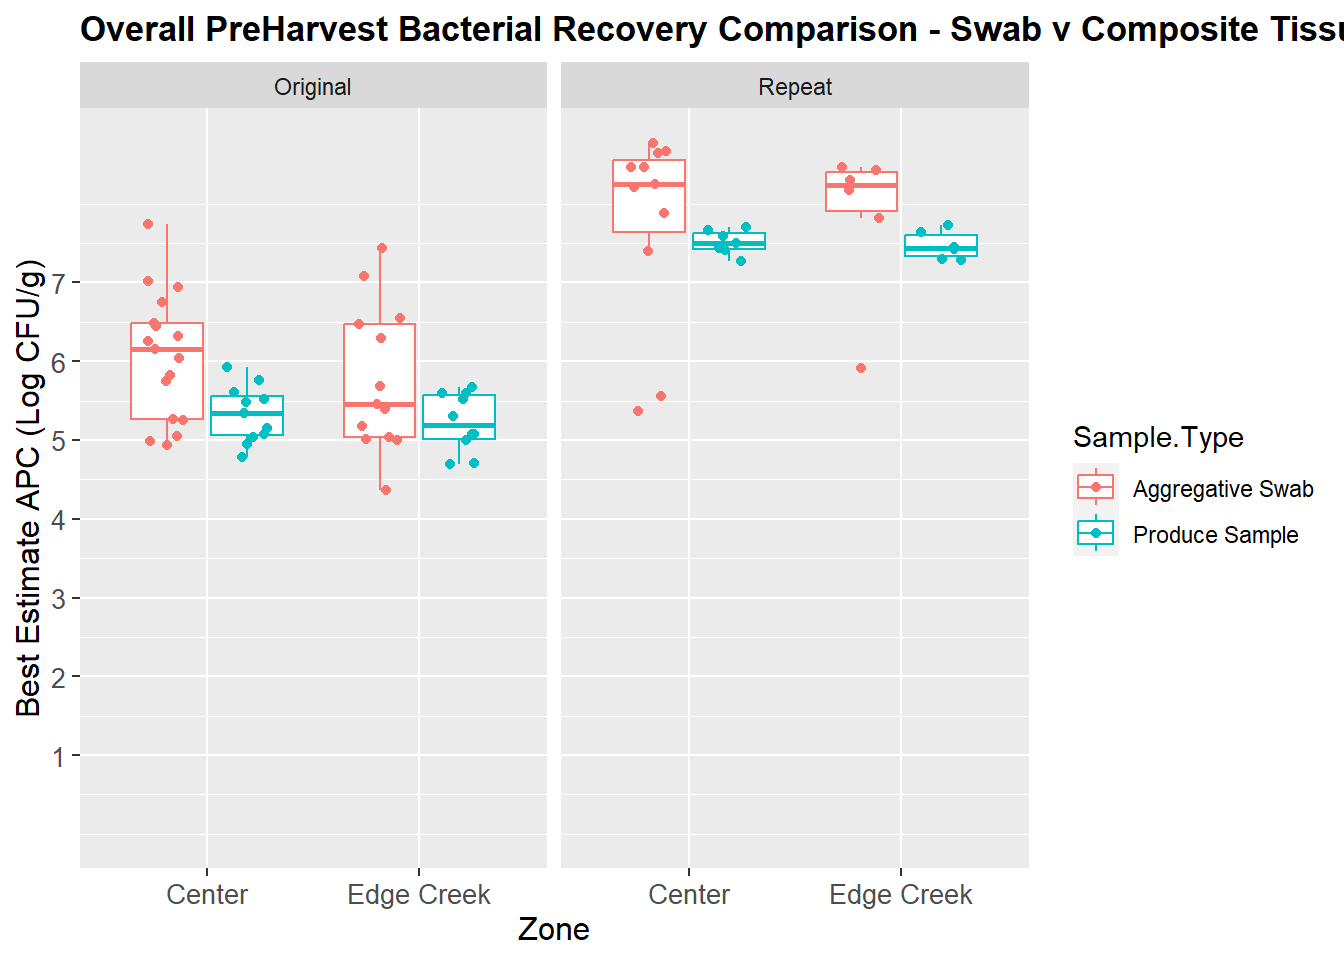
\includegraphics{Field-Trials-CA-2022_files/figure-latex/unnamed-chunk-3-1.pdf}
\emph{Overall, higher APC and Coliforms on repeated samples, why?}

\emph{\emph{However, following discussion on 07/11/22, we kept the
originals and filled in the gaps with the repeated samples}}

\begin{Shaded}
\begin{Highlighting}[]
\NormalTok{adj\_Fanoe}\OtherTok{\textless{}{-}}\FunctionTok{read.csv}\NormalTok{(}\StringTok{"Experiment\_1\_adjusted trim.csv"}\NormalTok{)}
\NormalTok{adj\_Fanoe}\SpecialCharTok{$}\NormalTok{Zone}\OtherTok{\textless{}{-}}\FunctionTok{as.factor}\NormalTok{(adj\_Fanoe}\SpecialCharTok{$}\NormalTok{Zone)}
\NormalTok{adj\_Fanoe}\SpecialCharTok{$}\NormalTok{Top.bottom}\OtherTok{\textless{}{-}}\FunctionTok{as.factor}\NormalTok{(adj\_Fanoe}\SpecialCharTok{$}\NormalTok{Top.bottom)}
\NormalTok{adj\_Fanoe}\SpecialCharTok{$}\NormalTok{Wet.dry}\OtherTok{\textless{}{-}}\FunctionTok{as.factor}\NormalTok{(adj\_Fanoe}\SpecialCharTok{$}\NormalTok{Wet.dry)}
\NormalTok{adj\_Fanoe}\SpecialCharTok{$}\NormalTok{Hand.msd}\OtherTok{\textless{}{-}}\FunctionTok{as.factor}\NormalTok{(adj\_Fanoe}\SpecialCharTok{$}\NormalTok{Hand.msd)}
\NormalTok{adj\_Fanoe}\SpecialCharTok{$}\NormalTok{Opportunity}\OtherTok{\textless{}{-}}\FunctionTok{as.factor}\NormalTok{(adj\_Fanoe}\SpecialCharTok{$}\NormalTok{Opportunity)}
\NormalTok{adj\_Fanoe}\SpecialCharTok{$}\NormalTok{Sample.Type}\OtherTok{\textless{}{-}}\FunctionTok{as.factor}\NormalTok{(adj\_Fanoe}\SpecialCharTok{$}\NormalTok{Sample.Type)}
\FunctionTok{str}\NormalTok{(adj\_Fanoe)}
\end{Highlighting}
\end{Shaded}

\begin{verbatim}
## 'data.frame':    54 obs. of  15 variables:
##  $ Samples.ID    : chr  "Tis8" "Tis59" "Tis4" "Tis22" ...
##  $ Sample.Type   : Factor w/ 2 levels "Aggregative Swab",..: 2 2 2 2 2 2 2 2 2 2 ...
##  $ Bed.number    : chr  "Edge Creek" "4" "Edge Creek" "1" ...
##  $ Hand.msd      : Factor w/ 2 levels "HAND","MSD": NA NA NA NA NA NA NA NA NA NA ...
##  $ Wet.dry       : Factor w/ 2 levels "DRY","WET": NA NA NA NA NA NA NA NA NA NA ...
##  $ Top.bottom    : Factor w/ 2 levels "Bottom","Top": 2 2 1 2 2 2 1 2 2 1 ...
##  $ Date.collected: chr  "6/27/2022" "6/27/2022" "6/27/2022" "6/27/2022" ...
##  $ Date.processed: chr  "6/29/2022" "6/29/2022" "6/29/2022" "6/29/2022" ...
##  $ Weight.g.     : num  214 439 811 400 417 ...
##  $ PBS.added.ml. : num  194 419 791 380 397 ...
##  $ Log.APC.      : num  5.67 5.76 5.3 5.15 4.95 ...
##  $ Log.Coli.     : num  6.12 5.83 4.26 4.62 4.08 ...
##  $ Log.E.coli.   : num  2.53 NA NA 3.15 2.3 ...
##  $ Opportunity   : Factor w/ 2 levels "Original","Repeat": 1 1 1 1 1 1 1 1 1 1 ...
##  $ Zone          : Factor w/ 2 levels "Center","Edge Creek": 2 1 2 1 1 1 2 2 2 1 ...
\end{verbatim}

\begin{Shaded}
\begin{Highlighting}[]
\NormalTok{wkngsamples\_Fanoe}\OtherTok{\textless{}{-}}\NormalTok{adj\_Fanoe}\SpecialCharTok{\%\textgreater{}\%}\FunctionTok{group\_by}\NormalTok{(Sample.Type, Wet.dry, Hand.msd)}\SpecialCharTok{\%\textgreater{}\%}\FunctionTok{summarise}\NormalTok{(}\AttributeTok{n=}\FunctionTok{n}\NormalTok{())}
\end{Highlighting}
\end{Shaded}

\begin{verbatim}
## `summarise()` has grouped output by 'Sample.Type', 'Wet.dry'. You can override
## using the `.groups` argument.
\end{verbatim}

\begin{Shaded}
\begin{Highlighting}[]
\NormalTok{totalecoli}\OtherTok{\textless{}{-}}\NormalTok{adj\_Fanoe}\SpecialCharTok{\%\textgreater{}\%}\FunctionTok{group\_by}\NormalTok{(Sample.Type, Log.E.coli.)}\SpecialCharTok{\%\textgreater{}\%}\FunctionTok{summarise}\NormalTok{(}\AttributeTok{count=}\FunctionTok{n}\NormalTok{())}
\end{Highlighting}
\end{Shaded}

\begin{verbatim}
## `summarise()` has grouped output by 'Sample.Type'. You can override using the
## `.groups` argument.
\end{verbatim}

\begin{Shaded}
\begin{Highlighting}[]
\NormalTok{knitr}\SpecialCharTok{::}\FunctionTok{kable}\NormalTok{(wkngsamples\_Fanoe)}
\end{Highlighting}
\end{Shaded}

\begin{longtable}[]{@{}lllr@{}}
\toprule\noalign{}
Sample.Type & Wet.dry & Hand.msd & n \\
\midrule\noalign{}
\endhead
\bottomrule\noalign{}
\endlastfoot
Aggregative Swab & DRY & MSD & 11 \\
Aggregative Swab & WET & HAND & 6 \\
Aggregative Swab & WET & MSD & 15 \\
Produce Sample & NA & NA & 22 \\
\end{longtable}

\begin{Shaded}
\begin{Highlighting}[]
\NormalTok{knitr}\SpecialCharTok{::}\FunctionTok{kable}\NormalTok{(totalecoli)}
\end{Highlighting}
\end{Shaded}

\begin{longtable}[]{@{}lrr@{}}
\toprule\noalign{}
Sample.Type & Log.E.coli. & count \\
\midrule\noalign{}
\endhead
\bottomrule\noalign{}
\endlastfoot
Aggregative Swab & 1.977724 & 1 \\
Aggregative Swab & 2.462398 & 1 \\
Aggregative Swab & 3.230449 & 1 \\
Aggregative Swab & 3.633469 & 1 \\
Aggregative Swab & 3.806180 & 1 \\
Aggregative Swab & 4.267606 & 1 \\
Aggregative Swab & NA & 26 \\
Produce Sample & 1.342423 & 1 \\
Produce Sample & 1.505150 & 1 \\
Produce Sample & 2.301030 & 1 \\
Produce Sample & 2.531479 & 1 \\
Produce Sample & 2.602060 & 1 \\
Produce Sample & 2.698970 & 1 \\
Produce Sample & 2.903090 & 1 \\
Produce Sample & 3.146128 & 1 \\
Produce Sample & 3.300000 & 1 \\
Produce Sample & NA & 13 \\
\end{longtable}

\textbf{Updated dataset consists on 32 swabs and 22 produce samples,
N=54. MSD Dry cloths n=11, Prehydrated cloths, hand n=6, Prehydrated
cloths, MSD n= 15.} \textbf{Generic \emph{E. coli} Neg swabs= 26, Pos
swabs= 6; Neg Produce= 13, Pos produce= 9}

\begin{verbatim}
## Warning: Removed 1 rows containing non-finite values (`stat_boxplot()`).
\end{verbatim}

\begin{verbatim}
## Warning: Removed 1 rows containing missing values (`geom_point()`).
\end{verbatim}

\includegraphics{Field-Trials-CA-2022_files/figure-latex/unnamed-chunk-5-1.pdf}
\includegraphics{Field-Trials-CA-2022_files/figure-latex/unnamed-chunk-5-2.pdf}

\hypertarget{including-plots}{%
\subsection{Including Plots}\label{including-plots}}

You can also embed plots, for example:

\includegraphics{Field-Trials-CA-2022_files/figure-latex/pressure-1.pdf}

Note that the \texttt{echo\ =\ FALSE} parameter was added to the code
chunk to prevent printing of the R code that generated the plot.

\end{document}
